\documentclass[12pt,a4paper]{ctexart}  
\usepackage[utf8]{inputenc}
\usepackage{easyReview}
\usepackage[T1]{fontenc}
\usepackage{amsmath}
\usepackage{fancyhdr}
\usepackage{amsfonts}
\usepackage{multirow}
\usepackage{booktabs}
\usepackage{subcaption}
\usepackage{float}
\usepackage{mathrsfs}
\usepackage{bm}
\usepackage{extarrows}
\usepackage{wasysym}
\usepackage{graphbox}
\usepackage{graphicx}
\usepackage[colorlinks,linkcolor=red,anchorcolor=blue,citecolor=green]{hyperref}
\usepackage{cases}
\usepackage{color}
\usepackage{tcolorbox}
\usepackage{listings}
\usepackage{xcolor}
\usepackage[framemethod=tikz]{mdframed}
\usepackage[left=2.00cm, right=2.00cm, top=2.00cm, bottom=2.00cm]{geometry}

\newcommand{\RNum}[1]{\uppercase\expandafter{\romannumeral #1\relax}}
\newtheorem{theorem}{定理}[section]
\newtheorem{lemma}[theorem]{Lemma}
\newtheorem{definition}[theorem]{定义}
\newtheorem{example}[theorem]{例}
\newtheorem{exercise}[theorem]{\textcolor{blue} {练习}}
\newtheorem{problem}[theorem]{问题}
\newtheorem{property}[theorem]{性质}
\newtheorem{proposition}[theorem]{命题}
\newtheorem{remark}[theorem]{Remark}
\newtheorem{algorithm}[theorem]{算法}

\pagestyle{fancy}
\cfoot{\thepage}
\lhead{{《最优化理论与方法》实验报告}}
\setlength{\headheight}{14.5pt}
\lstset{
    language=Python,
    basicstyle=\ttfamily\small,
    keywordstyle=\color{blue!70!black},
    commentstyle=\color{green!40!black},
    stringstyle=\color{red!60!black},
    numbers=left,
    numberstyle=\tiny\color{gray},
    stepnumber=1,
    frame=single,
    breaklines=true,
    showstringspaces=false,
    tabsize=4
}

\begin{document}

\vspace*{6em}
\begin{figure}[H]
	\centering
	
\includegraphics[width=0.4\linewidth]{picture/HNUlogo}
\end{figure}
\vspace*{4em}
\begin{center}
{\Huge \bf 《最优化算法与理论》 实验报告}
\end{center}
\vspace{4em}
\begin{center}
{\Large

{\bf\makebox[4em][s]{实验序号}}: \underline{\makebox[13em][c]{2}}\\
{\bf\makebox[4em][s]{实验内容}}: \underline{\makebox[13em][c]{下降算法比较}}\\
{\bf\makebox[4em][s]{班~~~~级}}: \underline{\makebox[13em][c]{信息2301}}\\
{\bf\makebox[4em][s]{学~~~~号}}: \underline{\makebox[13em][c]{202310040128}}\\
{\bf\makebox[4em][s]{姓~~~~名}}: \underline{\makebox[13em][c]{雷龙浩}}\\
{\bf\makebox[4em][s]{完成日期}}: \underline{\makebox[13em][c]{2026年03月29日}}\\

}
\end{center}
\clearpage

\tableofcontents
\newpage

\section{算法原理与实现概要}
\subsection{下降算法的一般迭代格式}
本次实验涉及的三类下降算法均遵循如下迭代形式：
\begin{equation}
x_{k+1} = x_k + \alpha_k d_k,
\end{equation}
其中 $d_k$ 为搜索方向，$\alpha_k>0$ 由线搜索确定。

\subsection{最速下降法（Steepest Descent）}
最速下降法取负梯度方向作为搜索方向：
\begin{equation}
d_k = -\nabla f(x_k).
\end{equation}
该方法实现简单、每步计算量小，但当目标函数等高线高度扭曲时，容易在谷底两侧来回摆动，从而出现典型的锯齿现象，整体收敛速度通常较慢。

\subsection{牛顿法（Newton Method）}
牛顿法利用二阶信息构造方向：
\begin{equation}
d_k = -[\nabla^2 f(x_k)]^{-1}\nabla f(x_k),
\end{equation}
实现中通常以求解线性方程组 $\nabla^2 f(x_k) d_k = -\nabla f(x_k)$ 的方式获得 $d_k$。
当 Hessian 正定且当前位置已经接近极小点时，牛顿法通常具有很快的局部收敛速度，因此在中小规模光滑问题中表现往往明显优于一阶方法。

\subsection{修正牛顿法（Modified Newton）与修正 Cholesky}
当 Hessian 非正定时，直接使用牛顿方向可能失去下降性，线搜索也可能无法接受该方向。
为此，修正牛顿法不直接求解
\[
\nabla^2 f(x_k) d_k = -\nabla f(x_k),
\]
而是先构造一个正定近似矩阵 $B_k$，再求解
\begin{equation}
B_k d_k = -\nabla f(x_k).
\end{equation}
本实验中的修正牛顿法采用课件中的修正 Cholesky 思想，将矩阵分解为
\[
B_k = L D L^T.
\]
其中每一列分解时，对角元按照
\[
d_j = \max\left\{|c_{jj}|,\left(\frac{\theta_j}{\beta}\right)^2,\delta\right\}
\]
进行修正，从而保证 $d_j>0$，最终保证 $B_k$ 为正定矩阵。这样做的直接效果是：即使原始 Hessian 含有负曲率信息，算法仍然可以构造出可靠的下降方向。

\section{实验设置}
\subsection{代码结构与运行方式}
本次实验的代码按模块化方式组织：
\begin{itemize}
  \item \texttt{optimization/core.py}：目标函数、梯度、Hessian 的统一封装；
  \item \texttt{optimization/line\_search/}：黄金分割、Armijo、Wolfe-Powell 三种线搜索；
  \item \texttt{optimization/optimizers/}：最速下降法、牛顿法、修正牛顿法；
  \item \texttt{work2/work2.py}：实验入口、结果打印与图片绘制。
\end{itemize}
在项目根目录运行
\begin{quote}
\texttt{python work2/work2.py}
\end{quote}
即可完成四组实验，并生成报告所需图片。

\subsection{主要参数设置}
\begin{table}[H]
\centering
\caption{实验中的主要参数设置}
\label{tab:work2_params_general}
\begin{tabular}{lccc}
\toprule
参数名称 & 符号 & 取值 & 说明 \\
\midrule
Rosenbrock/Rastrigin 停止阈值 & $\epsilon$ & $10^{-5}$ & 当 $\|\nabla f(x_k)\|\le \epsilon$ 时停止 \\
a9a 二阶法停止阈值 & $\epsilon$ & $10^{-6}$ & 为了更清楚比较二阶法精度表现 \\
修正 Cholesky 下界 & $\delta$ & 按课件公式自动计算 & 代码中取 $\delta=\epsilon_{\mathrm{mach}}\max(\gamma+\xi,1)$ \\
逻辑回归正则项 & $\lambda$ & $1/(100m)$ & $m$ 为样本数，防止过拟合 \\
\bottomrule
\end{tabular}
\end{table}

\subsection{线搜索参数设置}
\begin{table}[H]
\centering
\caption{线搜索参数}
\label{tab:work2_params_linesearch}
\begin{tabular}{lll}
\toprule
线搜索方法 & 参数配置 & 说明 \\
\midrule
Armijo & $\alpha_0=1,\ \rho=0.5,\ c_1=10^{-4}$ & 回溯收缩，保证充分下降 \\
Wolfe-Powell & $\alpha=1,\ \beta=0.5,\ c_1=10^{-4},\ c_2=0.9$ & 同时满足充分下降与曲率条件 \\
黄金分割 & $[a_k,b_k]=[0,2],\ \mathrm{tol}=10^{-4}$ & 一维精确线搜索 \\
\bottomrule
\end{tabular}
\end{table}

\subsection{关键代码展示}
由于完整代码较长，正文中只展示与本次实验最相关的两段核心实现。

\textbf{1. a9a 逻辑回归目标函数、梯度与 Hessian 定义}

\lstinputlisting[
    firstline=88,
    lastline=140,
    caption={work2.py 中逻辑回归目标函数的关键实现},
    label={lst:logistic-objective}
]{work2.py}

\textbf{2. 修正牛顿法中的修正 Cholesky 核心步骤}

\lstinputlisting[
    firstline=13,
    lastline=89,
    caption={modified\_newton.py 中修正 Cholesky 的关键实现},
    label={lst:modified-cholesky}
]{../optimization/optimizers/modified_newton.py}

\section{实验结果分析与讨论}
\subsection{Rosenbrock 函数最小化}
\textbf{函数形式：}
\begin{equation}
f(x)=100(x_2-x_1^2)^2+(1-x_1)^2.
\end{equation}
\textbf{问题特征：} Rosenbrock 函数存在一条狭长弯曲的香蕉形谷底，优化路径如果不能及时感知曲率变化，就会在谷底附近反复摆动，因此它非常适合用来比较一阶方法和二阶方法的差异。

\begin{table}[H]
\centering
\caption{Rosenbrock（$x_0=(1.2,1.2)$）三种下降法结果汇总}
\label{tab:work2_rosen_summary}
\begin{tabular}{lcccc}
\toprule
方法 & 迭代次数 & $f^\ast$ & 是否收敛 & $\|\nabla f(x^\ast)\|$ \\
\midrule
Steepest Descent & 10171 & $6.1958\times 10^{-11}$ & 是 & $9.87\times 10^{-6}$ \\
Newton Method & 7 & $3.2267\times 10^{-14}$ & 是 & $1.45\times 10^{-6}$ \\
Modified Newton & 7 & $3.2267\times 10^{-14}$ & 是 & $1.45\times 10^{-6}$ \\
\bottomrule
\end{tabular}
\end{table}

\begin{figure}[H]
\centering
\begin{subfigure}{0.48\linewidth}
  \centering
  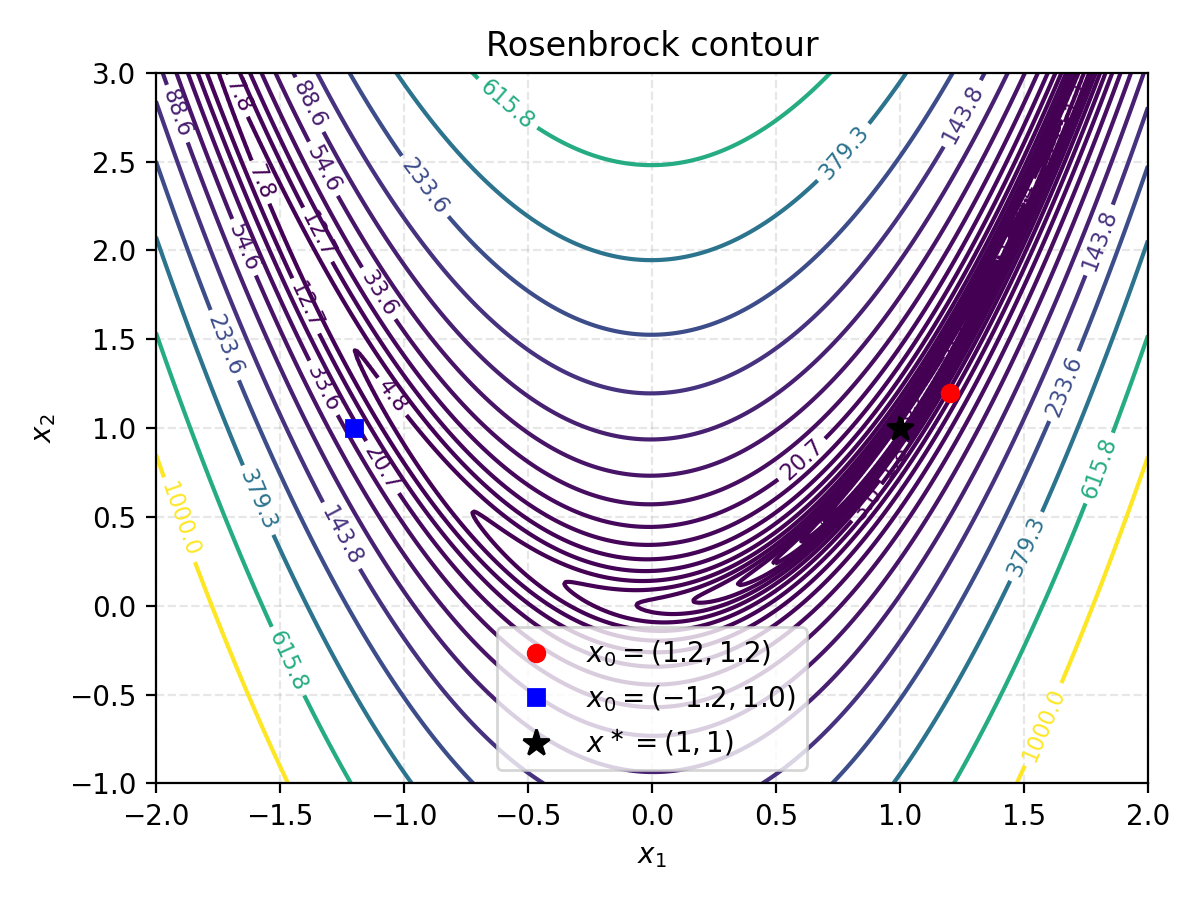
\includegraphics[width=\linewidth]{picture/rosenbrock_contour}
  \caption{Rosenbrock 等高线图}
\end{subfigure}
\hfill
\begin{subfigure}{0.48\linewidth}
  \centering
  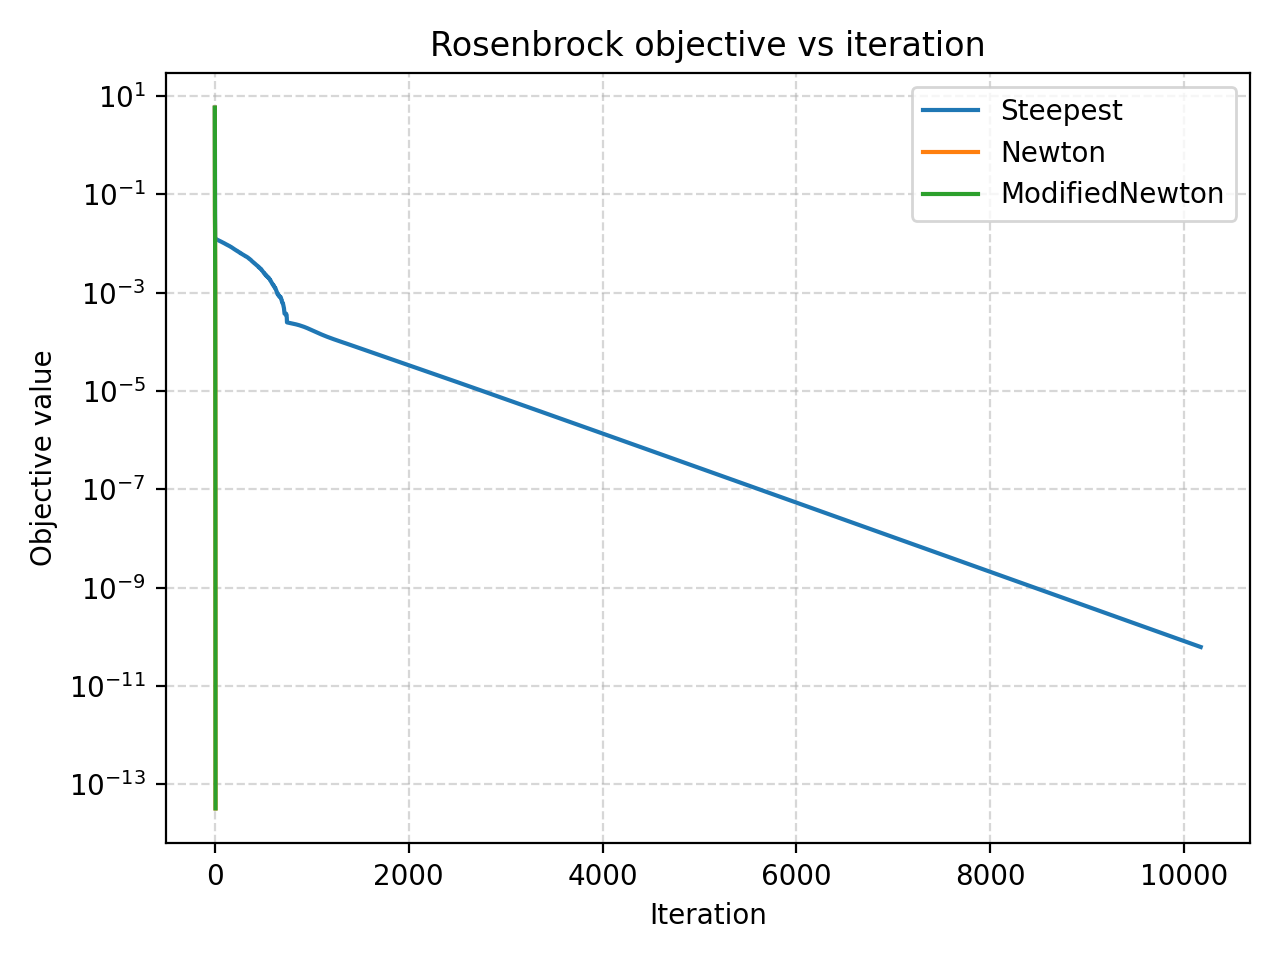
\includegraphics[width=\linewidth]{picture/rosenbrock_curve}
  \caption{目标函数值收敛曲线}
\end{subfigure}
\caption{Rosenbrock 问题的函数形状与收敛过程。}
\label{fig:work2_rosen_curve}
\end{figure}

结合上表和上图可以看出，最速下降法虽然最终也能收敛到极小点附近，但需要超过一万次迭代；与之相比，牛顿法和修正牛顿法都只用了 7 次迭代便达到较高精度，说明二阶曲率信息在该类病态问题中非常关键。
另外，在这个起点下牛顿法与修正牛顿法的轨迹完全一致，说明沿本次迭代路径 Hessian 的性质已经足够好，修正步骤没有显著改变方向。

\subsection{线搜索对迭代次数的影响（Rosenbrock，x0=(-1.2,1)）}
为了进一步观察步长策略的影响，固定初始点 $x_0=(-1.2,1)$，分别在三种下降法上使用黄金分割、Armijo 与 Wolfe-Powell 线搜索，结果见下表。

\begin{table}[H]
\centering
\caption{Rosenbrock（$x_0=(-1.2,1)$）线搜索对比结果}
\label{tab:work2_linesearch_compare}
\begin{tabular}{llccc}
\toprule
方法 & 线搜索 & 迭代次数 & $f^\ast$ & 是否收敛 \\
\midrule
Steepest Descent & Golden Ratio & 2409 & $1.2028\times 10^{-10}$ & 是 \\
Steepest Descent & Armijo & 10916 & $6.1319\times 10^{-11}$ & 是 \\
Steepest Descent & Wolfe-Powell & 10463 & $6.2082\times 10^{-11}$ & 是 \\
\midrule
Newton Method & Golden Ratio & 15 & $1.1657\times 10^{-16}$ & 是 \\
Newton Method & Armijo & 21 & $3.7440\times 10^{-21}$ & 是 \\
Newton Method & Wolfe-Powell & 21 & $3.7440\times 10^{-21}$ & 是 \\
\midrule
Modified Newton & Golden Ratio & 15 & $1.1650\times 10^{-16}$ & 是 \\
Modified Newton & Armijo & 21 & $3.7440\times 10^{-21}$ & 是 \\
Modified Newton & Wolfe-Powell & 21 & $3.7440\times 10^{-21}$ & 是 \\
\bottomrule
\end{tabular}
\end{table}

可以看到，线搜索策略对最速下降法的影响尤其显著：
在本例中，黄金分割法把迭代次数从约一万步降低到约两千四百步，效果非常明显。
对牛顿法与修正牛顿法而言，不同线搜索也会影响迭代次数，但影响幅度相对较小，
在这个二维光滑问题上，精确线搜索实现了更少的迭代次数。

\subsection{Rastrigin 函数与初始点敏感性}
\textbf{函数形式：}
\begin{equation}
f(x)=10n+\sum_{i=1}^{n}\left(x_i^2-10\cos(2\pi x_i)\right).
\end{equation}
\textbf{问题特征：} Rastrigin 函数具有强烈的周期振荡结构，局部极小点非常多，算法结果对起点和步长都比较敏感。下图给出了二维情形下的函数形状示意，虽然实际实验使用的是 $n=6$，但二维图足以反映其多峰特征。

\begin{table}[H]
\centering
\caption{Rastrigin（$n=6$）不同初始点下三种下降法结果}
\label{tab:work2_rastrigin}
\begin{tabular}{llccc}
\toprule
初始点编号 & 方法 & 迭代次数 & $f^\ast$ & 是否收敛 \\
\midrule
\#1 & Steepest Descent & 1 & $0.0000$ & 是 \\
\#1 & Newton Method & 2 & $5.3728\times 10^{1}$ & 是 \\
\#1 & Modified Newton & 2 & $5.3728\times 10^{1}$ & 是 \\
\midrule
\#2 & Steepest Descent & 1 & $0.0000$ & 是 \\
\#2 & Newton Method & 2 & $5.3728\times 10^{1}$ & 是 \\
\#2 & Modified Newton & 2 & $5.3728\times 10^{1}$ & 是 \\
\midrule
\#3 & Steepest Descent & 1 & $0.0000$ & 是 \\
\#3 & Newton Method & 1 & $0.0000$ & 是 \\
\#3 & Modified Newton & 9 & $2.7859\times 10^{1}$ & 是 \\
\bottomrule
\end{tabular}
\end{table}

\begin{figure}[H]
\centering
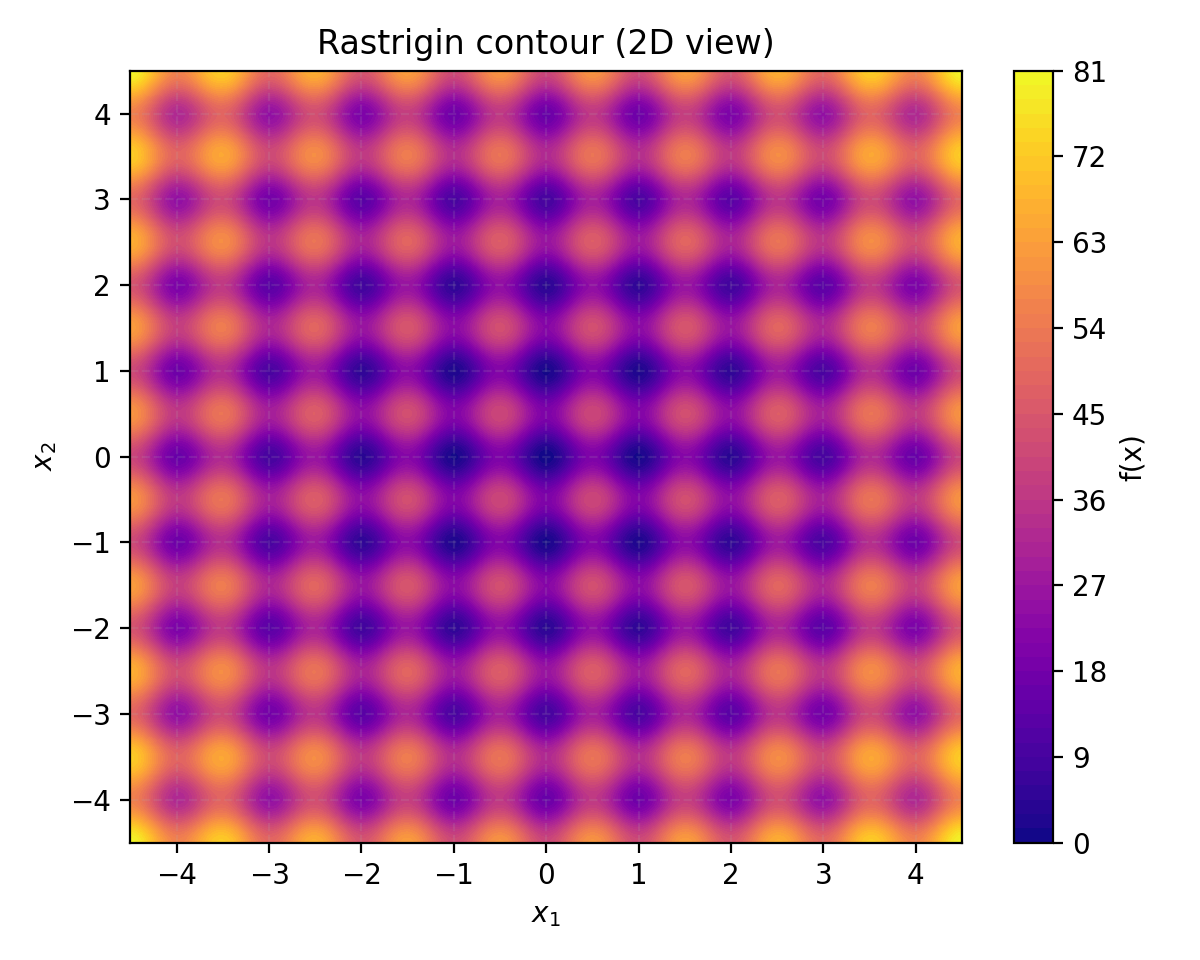
\includegraphics[width=0.62\linewidth]{picture/rastrigin_contour}
\caption{二维 Rastrigin 函数的等高线图（实验中实际使用 $n=6$，此图仅用于展示多峰结构）。}
\label{fig:work2_rastrigin_contour}
\end{figure}

从上表可以看到，不同算法和不同初始点的结果差异很大，这体现了非凸多峰问题的难度。
初始点 \#1 和 \#2 为例，最速下降法一步就到达了全局最优点附近，
而牛顿法和修正牛顿法却停在函数值约为 $53.728$ 的局部极小点；初始点 \#3 下，牛顿法得到全局最优，而修正牛顿法则停在函数值约为 $27.859$ 的另一个局部极小点。
这说明对于非凸问题，\textbf{收敛得快}与\textbf{收敛到全局最优}是两件不同的事情，牛顿类方法虽然局部收敛很快，但并不自动意味着全局结果更优。

\subsection{逻辑回归（a9a 数据集）性能对比}
\textbf{目标函数：}
\begin{equation}
\min_x\ \frac{1}{m}\sum_{i=1}^{m}\log\left(1+\exp(-b_i a_i^T x)\right)+\lambda\|x\|_2^2.
\end{equation}
\textbf{问题特征：} a9a 逻辑回归是一个典型的高维光滑优化问题。由于加入了 $L_2$ 正则项，目标函数具有较好的数值稳定性，也比较适合观察二阶方法在实际数据集上的表现。

\begin{table}[H]
\centering
\caption{a9a 逻辑回归三种下降法结果}
\label{tab:work2_logistic}
\begin{tabular}{lcccc}
\toprule
方法 & 迭代次数 & $f^\ast$ & 是否收敛 & $\|\nabla f(x^\ast)\|$ \\
\midrule
Steepest Descent & 2000 & $3.2295\times 10^{-1}$ & 否 & $1.906\times 10^{-4}$ \\
Newton Method & 7 & $3.2266\times 10^{-1}$ & 是 & $2.345\times 10^{-7}$ \\
Modified Newton & 7 & $3.2266\times 10^{-1}$ & 是 & $2.345\times 10^{-7}$ \\
\bottomrule
\end{tabular}
\end{table}

\begin{figure}[H]
\centering
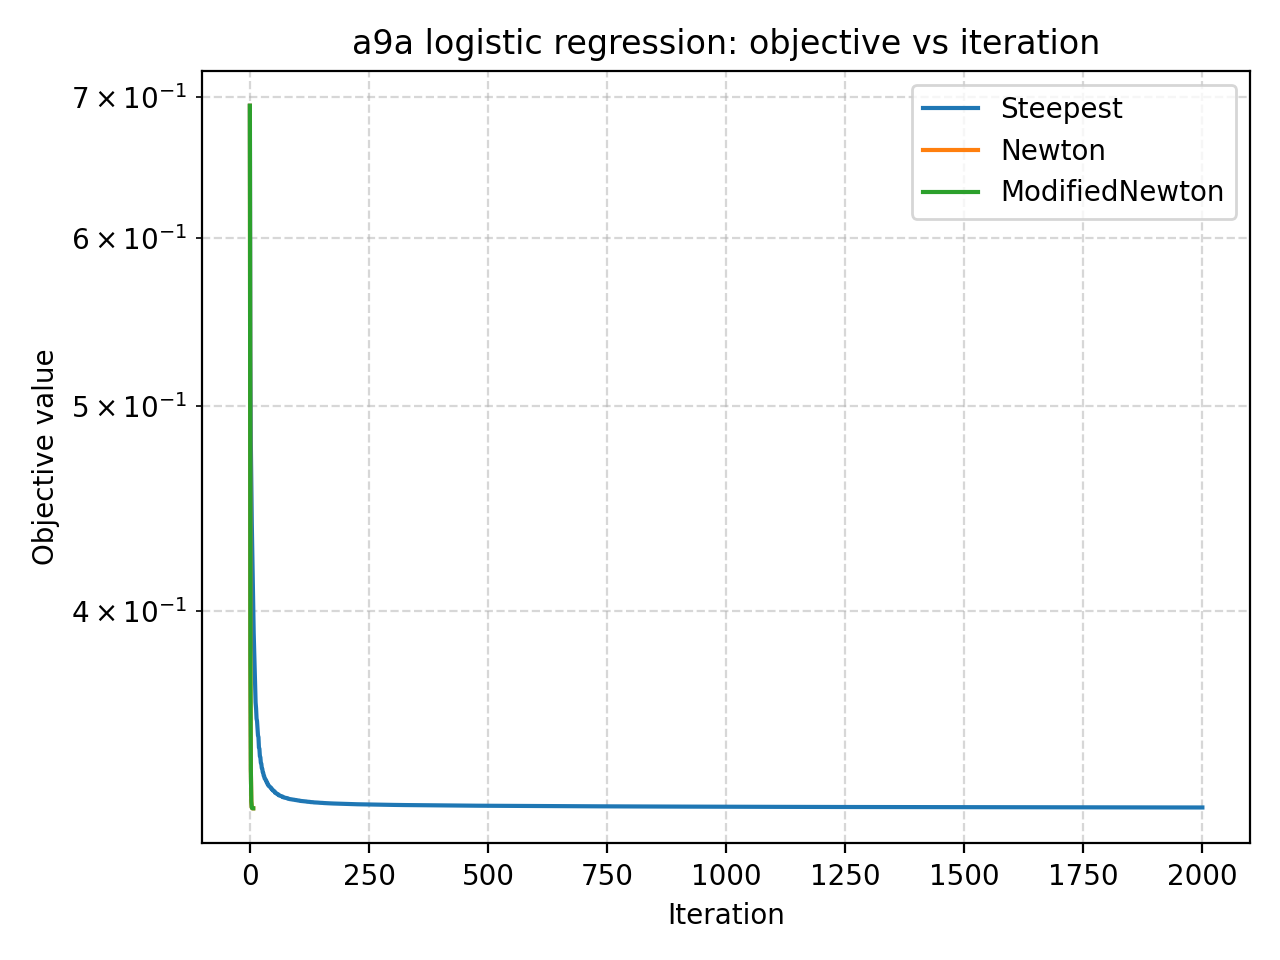
\includegraphics[width=0.72\linewidth]{picture/logistic_curve}
\caption{a9a 逻辑回归：目标函数值随迭代次数变化（半对数坐标）。}
\label{fig:work2_logistic_curve}
\end{figure}

结合上表和收敛曲线可以看出，最速下降法在达到 2000 次迭代上限后仍未满足停止条件，而牛顿法与修正牛顿法都只用了 7 步便收敛。
这里两种牛顿类方法结果完全一致，是因为逻辑回归加上二次正则后 Hessian 本身就是正定的，修正步骤没有触发。


\end{document}
